\documentclass[../main.tex]{subfiles}
\begin{document}

\section{Notation \& Definitions}

%% give the why of the math after every mention of why 
In this section we introduce a mathematical description of the visualization pipeline where artist $\mathscr{A}$ functions transform data space $\mathscr{E}$ to an intermediate representation in a prerendered graphic space $\mathscr{H}$. 

\begin{equation}
    \label{eq:artist}
    \mathscr{A}: \mathscr{E} \rightarrow \mathscr{H}
\end{equation}

We first describe how we model data(\ref{sec:data}), graphics(\ref{sec:graphic}), and intermediate visual characteristics (\ref{sec:artist}) as fiber bundles. We then discuss the equivariant maps between data and visual characteristics (\ref{sec:artist_nu}) and visual characteristics and graphics (\ref{sec:artist_q}) that make up the artist.

\subsection{Data Space}
\label{sec:data}
We build on Butler's proposal of using fiber bundles as a common data representation format for visualization data\cite{butlerVectorBundleClassesForm1992,butlerVisualizationModelBased1989} because fiber bundles are mathematical structures that are flexible enough to encode all the types of data described in section~\ref{sec:intro_data_structure} and many more. We model data as the fiber bundle $(E,\,B,\,\pi ,\,F)$, where $E$, $F$, and $K$ are topological spaces that encode 
\begin{itemize}
\item the properties of the variables in the fiber $F$ (\ref{sec:data_fiber})
\item the continuity of the records in the base space $K$ (\ref{sec:data_base})
\item collections of records $\tau$ (\ref{sec:data_section}). 
\end{itemize}

and $E$ is the total space of data that $F$ lives in. The bundle is the projection map $\pi$
\begin{equation}
    \label{eq:fiber_bundle}
    \begin{tikzcd}
        F \arrow[r, hook] & E \arrow[r, "\pi"] & K
    \end{tikzcd}
\end{equation}

that binds the variable space $F$ to the base space $K$. The fiber bundles mentioned in this work are assumed to be trivial\cite{spanier1989algebraic,LocallyTrivialFibre}, unless otherwise specified, because the trivial bundle is $E=K\times F$ such that extra structure in the total space $E$ falls out and discussion can be focused on the fiber and base space.

\begin{figure}[ht!]
    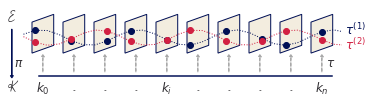
\includegraphics[width=1\linewidth]{figures/math/fiberbundle.png}
    \label{fig:data_base_space}
    \caption{}.  
\end{figure}
 We propose fiber bundles as an underlying data representation because they provide a way to decouple the components of a dataset. In figure~\ref{fig:}, we have two datasets $\tau_1$ and $\tau_2$ that have the same indexing structure $K$ and and the same schema $F$ and we can independently codify which properties of each component need to be preserved in the visualization.

\subsubsection{Variables: Fiber Space $F$}
\label{sec:data_fiber}
We use Spivak's description of schemas in his categorical formulation of databases \cite{spivakSIMPLICIALDATABASES} as our fiber space. He describes the variables in a dataset as having names $C$ and datetypes $D$. Spivak then constructs a set $U_{\sigma}$ that is the universal set of values 
\begin{tikzcd}
    U_{\sigma} \arrow[r] \arrow[d, "\pi_{\sigma}"'] & U \arrow[d, "\pi"] \\
    C \arrow[r, "\sigma"']                          & \textbf{DT}       
\end{tikzcd}

restricted to values of types $\mathbf{DT}$ bound to variable names $C$. Therefore the fiber is for a one variable dataset is
\begin{equation}
    F = U_{\sigma}
\end{equation}
where $\sigma$ is the schema binding variable name to variable type. Therefore a dataset with multiple variables $c \in C$ has a fiber that is the cartesian cross product of $U_{\sigma}$ restricted over $c$ spaces:

\begin{equation}
F = U_{\sigma(c_1)}\times \ldots U{\sigma{c_i}} \ldots\timesU_{sigma(c_n)}
\end{equation}

which is equivalent to 

\begin{equation}
    F= F_{0} \times \ldots \times F_{i}\times\ldots\times F_{n}
\end{equation}


%%somehoe close out this piece. 



For example, a fiber $F$ that is the temperature variable from GHCN is the range of physically possible temperature values $ U_{temp} = \{x \in \mathbb{R}^+\}$. 
\begin{equation}
    F = U_{temp}
\end{equation}
Then lets add the time variable from GHCN $U_{time} = \{x \in \mathbb{R}^+\}$ 
\begin{equation}
F =  U_{temp} \times U_{time}
\end{equation}
such that $F$ is the cartesian product of $F_0=U_{temp}$ and $F_1 = U_{time}$. The elements in a given fiber set do not need to be scalers; for example the location of each record can be encoded as $U_{loc} = \{y, x \in \mathbb{R}^{2} \mid -90^\circ \leq y \leq 90^\circ, -180^\circ \leq x -180^\circ\}$: %add comment about latitude and longitude
\begin{equation}
    F = U_{temp} \times U_{time} \times U_{loc}
\end{equation}
such that one record $r$ in the fiber would have the form $r=(temperature,\, time,\, (latitude,\, longitude))$. We also add the variable name and measurement scale $M$ monoid actions to the fiber $F_i$ such that 
\begin{align}
    F_0 &= (\textit{temperature},\, U_{temp},\, M_0)\\
    F_1 &= (\textit{time},\, U_{time},\, M_1)\\
    F_2 &= (\textit{location},\, U_{loc},\, M_2)
\end{align}

%%invert this section, start w/ general math than GHCN 

\subsubsection{Measurement Scales: Monoid Actions}
\label{sec:data_monoid}

\begin{figure}[ht!]
    
\includegraphics[width=\textwidth]{figures/math/rotation_actions.png}
    \label{fig:data_monoid_rotation}
    \caption{The set of rotation actions [turn 0, 90, 180] on the star produce a star (closed), include a rotation that does not change the orientation (identity), and can be done in any order to produce the same final orientation (closure); therefore the rotations are a set of monoid actions.
    %% dataset that is symmetric, fiber is x,y, rotatation action
    %% rotate + plot or plot + rotate
    %%emoji shuffle 
    }  
\end{figure}

A common task is modifying the values in $F_i$ in some consistent way, such as converting data from \textdegree F to \textdegree C or changing category labels or rotating a shape such as in figure~\ref{fig:data_monoid_rotation}. This model formally encodes the set of allowable operations in the fiber because a transformation on the data side needs to be reflected in the visual representation, discussed in more detail in section~\ref{sec:artist_nu}.

We generalize the set of allowable transformations to the monoid actions $M_i$ on $F_i$. A monoid \cite{Monoid2021} $M_i$ is a set with an associative binary operator $\ast:M_i \times M_i\rightarrow M_i$. A monoid has an identity element $e\in M_i$ such that $e\ast a= a \ast e = a$ for all $a \in M_i$. A left monoid action \cite{SemigroupAction2021,ActionNLab} of $M_i$ is a set $U_{type}$ with an action $\bullet: M\times U_{type} \rightarrow U_{type}$ with the properties:
\begin{align*}
    \textbf{associativity}\;& \text{for all } m,t \in M \text{ and } x\in U_{type}, m\bullet(t\bullet x) = (m\ast t) \bullet x\\
    \textbf{identity}\;& \text{for all } x\in U_{type}, e\in M,  e\bullet x = x 
\end{align*}
As with the fiber $F$, the total monoid space $M$ is the cartesian product
\begin{equation}
M = M_{0} \times \ldots \times M_{i}\times \ldots \times\ldots M_{n}
\end{equation}
of the monoid $M_{i}$ on each $F_{i}\in F$. 

Steven's defined the measurment scales \cite{stevensTheoryScalesMeasurement1946,leaFormalizationMeasurementScale} in terms of the monoid actions permissible on the measurments; nominal data is permutable, ordinal data is monotonic, interval data is translatable, and ratio data is scalable \cite{weissteinSimilarityTransformation}. 

For example, the temperature in \textdegree C is on an interval scale, which means that the monoid actions $M_0$ on $U_{temp}$ are the set of translations $\{f: x\mapsto x + c \in U_{temp} \mid x,c \in U_temp\}$ where $c$ is a valid interval between two temperatures $c=x_i-x_j$.

\subsubsection{continuity: Base Space $K$} 
%%fold butlder
\label{sec:data_base}
The base space $K$ provides a way to encode how the records are connected to each other; for example the GHCN data can be expressed as discrete observations, many timeseries, maps, a network of stations, etc.

\begin{figure}[ht!]
    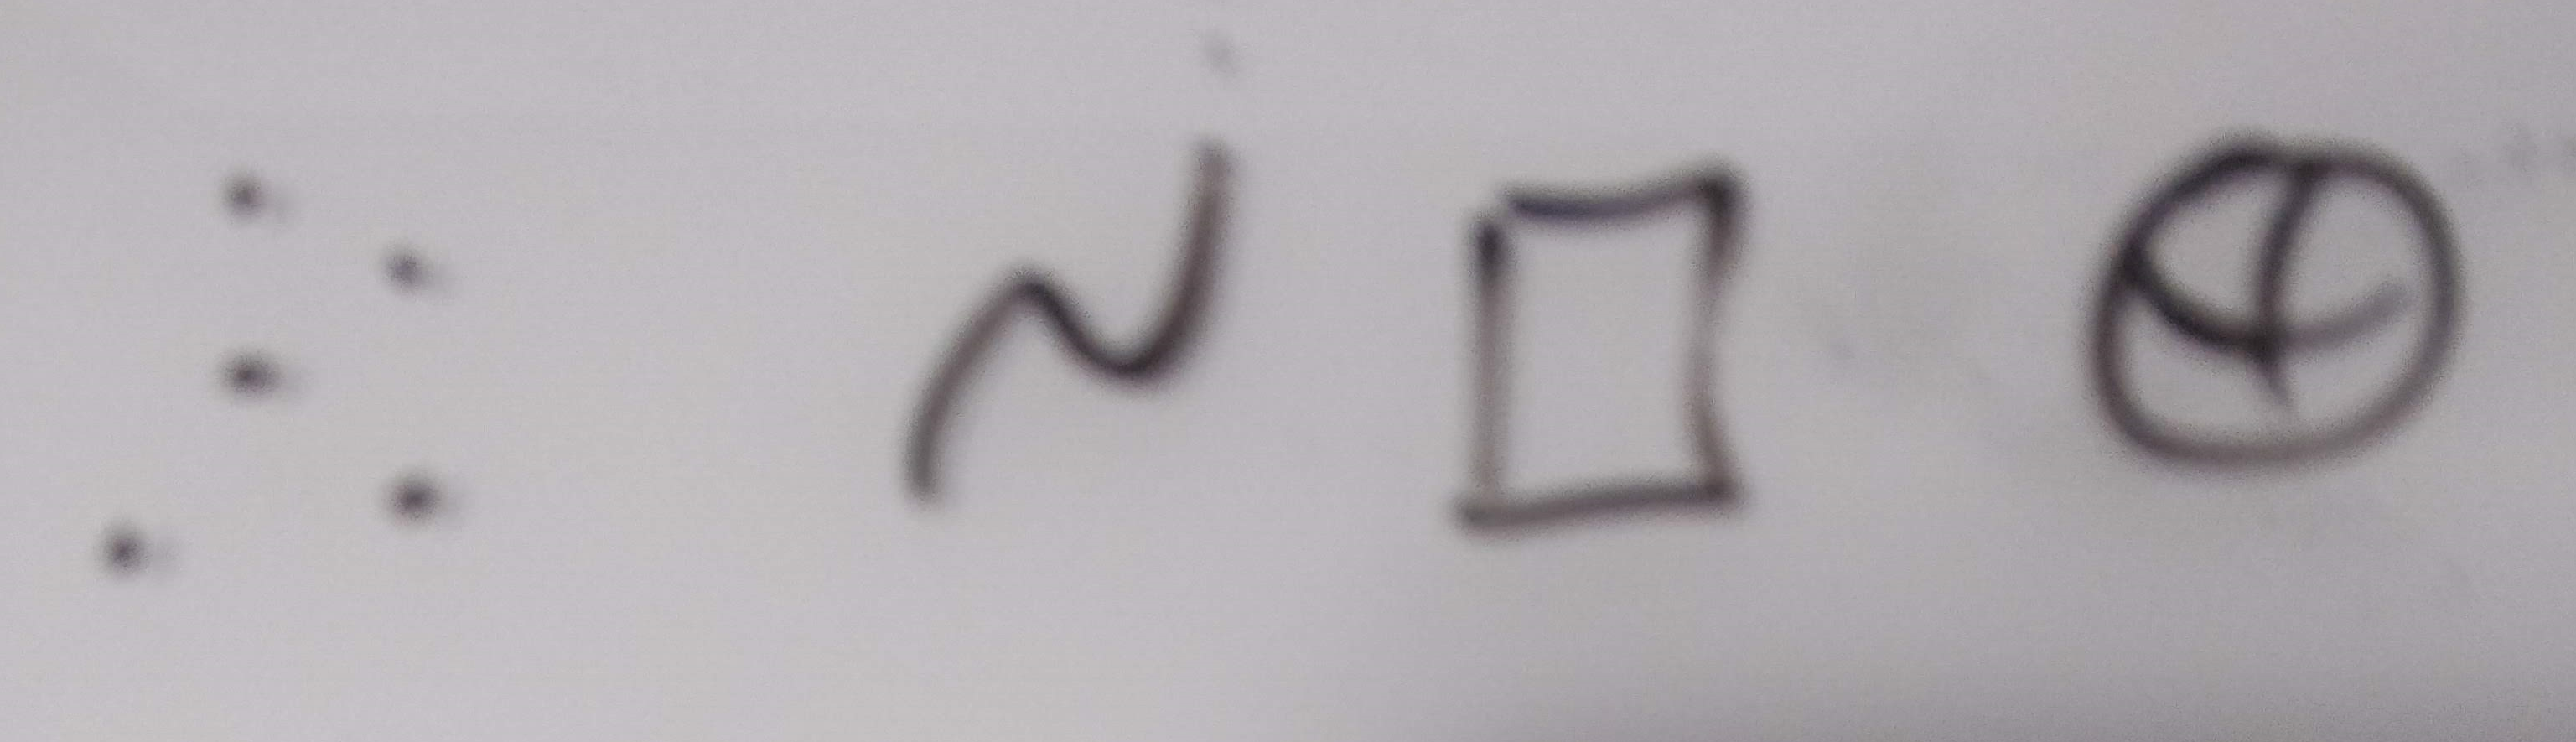
\includegraphics[width=.5\textwidth]{figures/math/k_different_types.png}
    \label{fig:base_space_types}
    \caption{The topological base space $K$ encodes the connectivity of the data space, for example if the data is independent points or a map or on a sphere}
\end{figure}

$K$ has no knowledge of the records. As illustrated in figure~\ref{fig:base_space_div}, $K$ is more of an indexing space into $E$ that describes the structure of $E$ and itself can be any number of dimensions. 

\begin{figure}[ht!]
    \label{fig:base_space_div}
    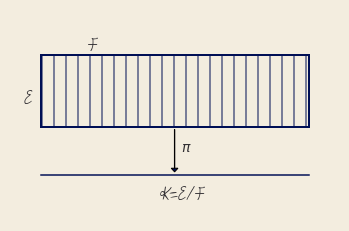
\includegraphics[width=.5\linewidth]{figures/math/k_qspace.png}
    \caption{ The base space $E$ is divided into fiber segments $F$. The base space $K$ acts as an index into the fibers.}
\end{figure}

Formally $K$ is the quotient space \cite{QuotientSpaceTopology2020} of $E$, meaning it is the finest space such that every $k \in K$ has a corresponding fiber $F_k$ in $E$. In figure~\ref{fig:base_space_div}, $E$ is a rectangle divided by vertical fibers $F$, so the minimal $K$ for which there is always a mapping $\pi: F\rightarrow K$ is the line. 


As with fibers and monoids, we can decompose the total space into components $\pi:E_i\rightarrow K$ where
\begin{equation}
    \pi:E_1\oplus\ldots\oplus E_i \oplus\ldots \oplus E_n \rightarrow K
\end{equation}

which is a decomposition of $F$. The $K$ remains the same because the connectivity of records does not change just because there are fewer elements in each record.

\subsubsection{Values: Sections $\tau$}
\label{sec:data_section}
\begin{figure}[ht!]
    \label{fig:base_space_div}
    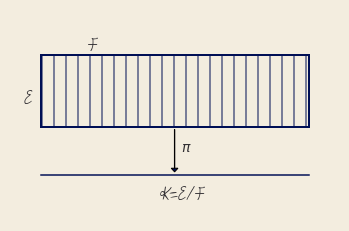
\includegraphics[width=.5\linewidth]{figures/math/k_qspace.png}
    \caption{ A section $\tau$ is a mapping from $K$ to $F$ that returns a record for each $k \in K$.}
\end{figure}

The sections of the fiber bundle are maps from points $k$ on $K$ to records $r$ in $F$. When we map our data to visual variables, the $\tau$ returns the set of values that are mapped together into a single graphic element. The section $\tau$ is the mapping from base space to total space $\tau: K\rightarrow E$ 
\begin{equation}
    \label{eq:section}
    \begin{tikzcd}
        F \arrow[r, hook] & E \arrow[d, "\pi"']           \\
        & K \arrow[u, "\tau"', bend right]
    \end{tikzcd}
\end{equation}
such that there is $\pi(\tau(k)) = k$ map back to $K$. 

A fiber bundle is trivial if $E = K\times F$\cite{rowlandFiberBundle,FiberBundle2020}.
All fiber bundles are locally trivial, which means if you restrict $E$ over a small enough neighborhood $U \subset K$ then it is a locally trivial bundle over $U$.
When the fiber bundle is locally trivial, then
\begin{equation}
    \label{eq:section_return}
    \tau(k) = (k, (g_{F_{0}}(k), \ldots, g_{F_{n}}(k))
\end{equation}
the section $\tau$ is the record in the $F$. Because we can decompose the bundle and the fiber, we can formulate $\tau$ as 
\begin{align}
\tau = (\tau_0,\ldots, \tau_i, \dots, \tau_n) 
\end{align}
where each section $\tau_i$ is a variable or set of variables. 

\paragraph{Example?}
For GHCN, the $\tau$ functions return a table in a database with the schema defined in $F$ and the continuity defined in $K$: this means the sections can be defined such that all values have the same year or location, e.g each table returned by a $\tau$ is for a different station. 

\subsubsection{Sheaf and Stalk}
\label{sec:data_sheaf_stalk}
%%% sheaf is how we break up the base space 
Often a graphic may need to be updated with live data or support zooming in on a segement of the dataset; to support working with a subset of data, we can use the sheaf $\mathcal{O}(E)$

\begin{equation}
    \label{eq:sheaf}
    \begin{tikzcd}
        \iota^*E \arrow[d, "\pi"']           & E \arrow[d, "\pi"'] \arrow[l, "\iota^*"']         \\
        U \arrow[u, "\iota^*\tau"', bend right] & K \arrow[u, "\tau"', bend right] \arrow[l, "\iota"']
        \end{tikzcd}
\end{equation}
which is the localized section of fibers $\iota^*\tau: U \rightarrow \iota^*E$ pulled back via the inclusion map $\iota: U \rightarrow K$. The localized section is the germ $\xi^*\tau$. The neighborhood of points $k_i$ surrounding the point $k$ the sheaf lies over is the stalk $\mathcal{F}_b$ \cite{StalkSheaf2019,spanier1989algebraic}.

%% the stalk contains all the local information, typically we only need some of the information, such as the firtst or second direivative. in practice we only need the jet which is...in practive will extend the fiber /fatten the E , notatoe E' = E + Jet
The jet bundle $\mathcal{J}$ \cite{JetBundle2020,musilovaCalculusVariationsJet2016} is for writing differential equations on sections of fiber bundles; this information is required for some visual characteristics, such as line thickness. 

\subsection{Prerender Space $H$}
\label{sec:graphic}
We define a graphic space $H$ such that we do not have to assume the physical output space of the renderer. This means that the graphic in $H$ can be output to a screen or 3D printed space or a dome. We model the prerender space as a fiber bundle (H, S, $\pi$, D). $H$ is the predisplay space, with a fiber $D$ dependent on the target display and a base space of $S$. 

%%define a region b = [top, bottom, right, left]
%% inverse of b is capital S_b
\subsubsection{Base space}
The underlying topology $S$ of a graphic often needs more dimensions than the data topology $K$ because of the specifications of the display space. For example, a line plot on a plane (such as a screen or a piece of paper) by necessity needs to also have a thickness so that it is visible, which maps back to a set of connected points in $H$. The topology of these connected points is therefore the region $s \subset S$ such that $\xi: S \rightarrow K$ is a deformation retraction \cite{RetractionTopology2020}
\begin{equation}
    \begin{tikzcd}
        E \arrow[d, "\pi"'] & H \arrow[d, "\pi"'] \\
        K                   & S \arrow[l, "\xi"']
        \end{tikzcd}
\end{equation}

that goes from a region $s \in S_{k}$ to its associated point $k$, such that when $\xi(s) = k$, $\xi^*\tau(s) = \tau(k)$. 

\subsubsection{Fiber and Section}
A section $\rho: S \rightarrow H$ is a mapping from a region $s$ on a mathematical encoding of the image to a region $xy$ on the screen that the renderer then maps to visual space as defined in D.

\paragraph{Example}
For a physical screen display, we can consider a predisplay space that is a trivial fiber bundle $H=\mathbb{R}^{5}\times S$ such that $\rho$ is
\begin{equation}
    \rho(s)  = (D_x(s), D_y(s), D_r(s), D_g(s), D_b(s))
    \label{eq:rho}
\end{equation}

To draw an image, a region, $H$ is inverse mapped into a region $s \in S$ where %%% 
\begin{equation}
s = \rho^{-1}_{\tiny{XY}}(xy)
\end{equation}
such that the rest of the fields in $\mathbb{R}^{7}$ are then integrated over $s$ to yield the remaining fields
%% redefining notation 
\begin{align}
    R_b &= \iint\limits_s D_r(s)ds^{2}\\
    G_b &= \iint\limits_s D_g(s)ds^{2}\\
    B_b &= \iint\limits_s D_b(s)ds^{2}
\end{align}

Here we assume a single opaque 2D image such that the $z$ and $alpha$ fields can be omitted. To support overplotting and transparency, we can consider $D=R^{7}$

\subsubsection{{Example}}
\begin{figure}[ht!]
    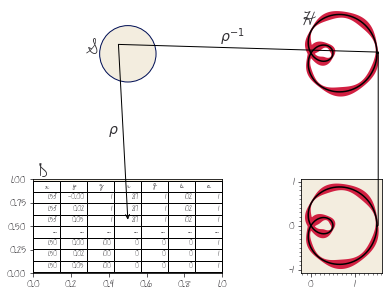
\includegraphics[width=.4\linewidth]{figures/math/render.png}
    \caption{}
    \label{fig:render}
\end{figure}

As illustrated in figure~\ref{fig:render}, words.

\subsection{Artist}
\label{sec:artist}

%% E' not E
In this section we will define the artist as a mapping from a sheaf $\mathcal{O}(E)$  to $\mathcal{O}(H)$. 
\begin{equation}
    A: \mathcal{O}(E) \rightarrow \mathcal{O}(H)
\end{equation}

The artist decomposes to mapping data to visual $\nu:E\rightarrow V$, then  compositing $V$ pulled back along $\xi$ to $\xi^*V$ to a visual mark in prerender space $Q:\xi^*V\rightarrow H$. 

\begin{equation}
    \label{eq:artist_diagram}
    \begin{tikzcd}
        E \arrow[r, "\nu"] \arrow[rd, "\pi"'] & V \arrow[d, "\pi"] & \xi^*V \arrow[r, "Q"] \arrow[d, "\xi^*\pi"'] \arrow[l, "\xi^*"'] & H \arrow[ld, "\pi"] \\
                                              & K                  & S \arrow[l, "\xi"']                                              &                    
        \end{tikzcd}
\end{equation}
The pullback map $\xi^*$ copies each value in $V$ over $k$ to $s$ in corresponding $S_k$ such that $\xi^*V$ can have multiple values that map to one value in $V$. 

The visual fiber bundle ($V$, $K$, $\pi$, $P$) has section $\mu: V \rightarrow K$ that resolves to a visual variable \cite{bertinIIPropertiesGraphic2011,munznerMarksChannels,} in fiber $P$. The visual transformer $\nu$ is a set of functions each targeting a different $\mu$
\begin{equation}
    \label{eq:nu_expanded}
    \{\nu_{0}, \ldots, \nu_{n}\}: \{\tau_{0}, \ldots, \tau_{n}\} \mapsto \{\mu_{0}, \ldots, \mu_{n}\}
\end{equation}

where $\mu_{i}$ are the visual parameters in the assembly function $Q(\mu_{0}, \ldots, \mu_{n})(s) = \rho(s)$. 


\subsubsection {Example: Matplotlib Visual Fiber}
For example, for Matplotlib \cite{hunterMatplotlib2DGraphics2007}, some of the possible types in $P$ are:
\begin{table}[ht]
    \renewcommand{\arraystretch}{2}
    \begin{tabulary}{\textwidth}{|l|L|l|}\hline
     $\bm{\nu_{i}}$                      & $\bm{\mu_{i}}$                                                            & $\bm{codomain(\nu_{i})}$  \\ \hline                                              
    position                    & x, y, z, theta, r                                                          & $\mathbb{R}$   \\ \hline
    size                        & linewidth, markersize                                            & $\mathbb{R}^{+}$   \\ \hline
    shape                       & markerstyle                                                      & $\{f_{0}, \ldots, f_{n}\}$ \\ \hline
    color                       & color, facecolor, markerfacecolor, edgecolor  & $\mathbb{R}^{4}$ \\ \hline
    \multirow{2}{*}{texture}    & hatch                                                            & $\mathbb{N}^{10}$\\\cline{2-3}
                                & linestyle                                                        & $\{f_{0}, \ldots, f_{n}\} \times (\mathbb{R}, \mathbb{R^+}^{n, n\%2=0})$ \\ \hline              
    \end{tabulary}
    \label{tab:mpl_visual_variable_fiber}
\end{table}

Table~\ref{tab:mpl_visual_variable_fiber} is an example of the visual fiber defined in terms of common parameters to plots in Matplotlib. The range of $\mu_{i}$ determine the monoid actions on $\mu_{i}$. A section of V $\mu$ is a tuple of visual values that specifies the visual characteristics of a glyph. For example, given a fiber of $\{xpos, ypos, color\}$ one section is $\{.5, .5, (255, 20,147)\}$. $Q$ determines how this section is applied to a graphic.  

\subsubsection{Visual Channels}
\label{sec:artist_nu}
$\nu: E \rightarrow V$ is an equivariant map such that there is a homomorphism from left monoid actions on $E_{i}$ to left monoid actions on $V_{i}$ where $i$ identifies a field in the fiber. $E_i$ and $V_{i}$ each contain a set of values as defined in $F$ and $P$ respectively. A validly constructed $\nu$ is one where the  diagram 
\begin{equation}
    \label{eq:nu_categorical}
\begin{tikzcd}
    E_i \arrow[r] \arrow[r, "\nu_i"] \arrow[d, "m_e"'] & V_i \arrow[d, "m_v"] \\
    E_i \arrow[r, "\nu_i"]                           & V_i               
\end{tikzcd}
\end{equation}
commutes such that $\nu_i(m_e(E_i)) = m_v(\nu_i(E_i))$.

\paragraph{Example: Ordering}
To preserve ordering of elements in $E_i$, $\nu$ must be a monotonic function such that given $e_1, e_2 \in E_{i}$
\begin{equation}
\text{ if } e_1 \leq e_2 \text{ then } \nu(e_1) \leq \nu(e_2)
\end{equation}

\paragraph{Example: Translation}
According to Stevens, interval data is a set with general linear group actions \cite{stevensTheoryScalesMeasurement1946,leaFormalizationMeasurementScale}. Position is a visual variable that can support translation 
\begin{equation}
\nu(x + c) = \nu(x) + \nu(c)
\end{equation}


\paragraph{Example: Invalid $\nu$}
Given a transform $t(x) = x+2$, we construct a $\nu$ that always takes data to .5: 
\begin{equation}
    \label{eq:nu_equation_bad}
    \begin{tikzcd}
        E_1 \arrow[r] \arrow[r, "\lambda:e\mapsto.5"] \arrow[d, "2e"'] & V_i \arrow[d, "2v"] \\
        E_1 \arrow[r, "\lambda"]                                        & V_1                 
    \end{tikzcd}
\end{equation}

This $\nu$ is invalid because the graph does not commute for $t$:
\begin{align}
    \nu(t(e)) & \overset{?}{=} t(\nu(e))\\
    .5 & \overset{?}{=} t(.5)\\
    .5 & \neq 2*.5
\end{align}

To construct a valid $\nu$, the diagram must commute for all monoid actions on the sets in $E_i, V_i$.


\subsubsection{Assembling Marks}
\label{sec:artist_q}
\begin{figure}[ht!]
    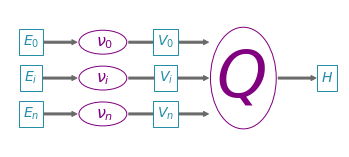
\includegraphics[width=\textwidth]{figures/math/path_of_q}
    \label{fig:artist_q}
    \caption{The $\nu$ functions convert data $E$ to visual $V$. $Q$ assembles the different types of visual parameters $V_{i}$ into a graphic in $H$. $Q\circ\mu(\xi^{-1}J)$ forms a visual mark by applying $Q$ to a region mapped to connected components $J \subset K$.}
    %%maybe change to \tau, \mu, \rho  
\end{figure}

As shown in figure~\ref{fig:artist_q}, $Q$ takes the individual fields in $V$ as input and outputs a single piece of a graphic on $H$. As with $\nu$, the constraint on $Q$ is that for every monoid actions on the input in $V$ there is a corresponding monoid action on the output in $H$
\begin{equation}
    Q: \Gamma(V) \rightarrow \Gamma(H)
\end{equation}
When $Q: \mu \mapsto \rho$ yields a $\rho$ that maps to the same values in $D$ over all $S_k$, then $M$ can be defined over $\Gamma(H)$ such that a constraint on $Q$ is that it must be equivariant. For example, when $\mu_{i}$ is the color of the glyph, it maps directly to (R,G,B) in D.

\begin{figure}[ht!]
    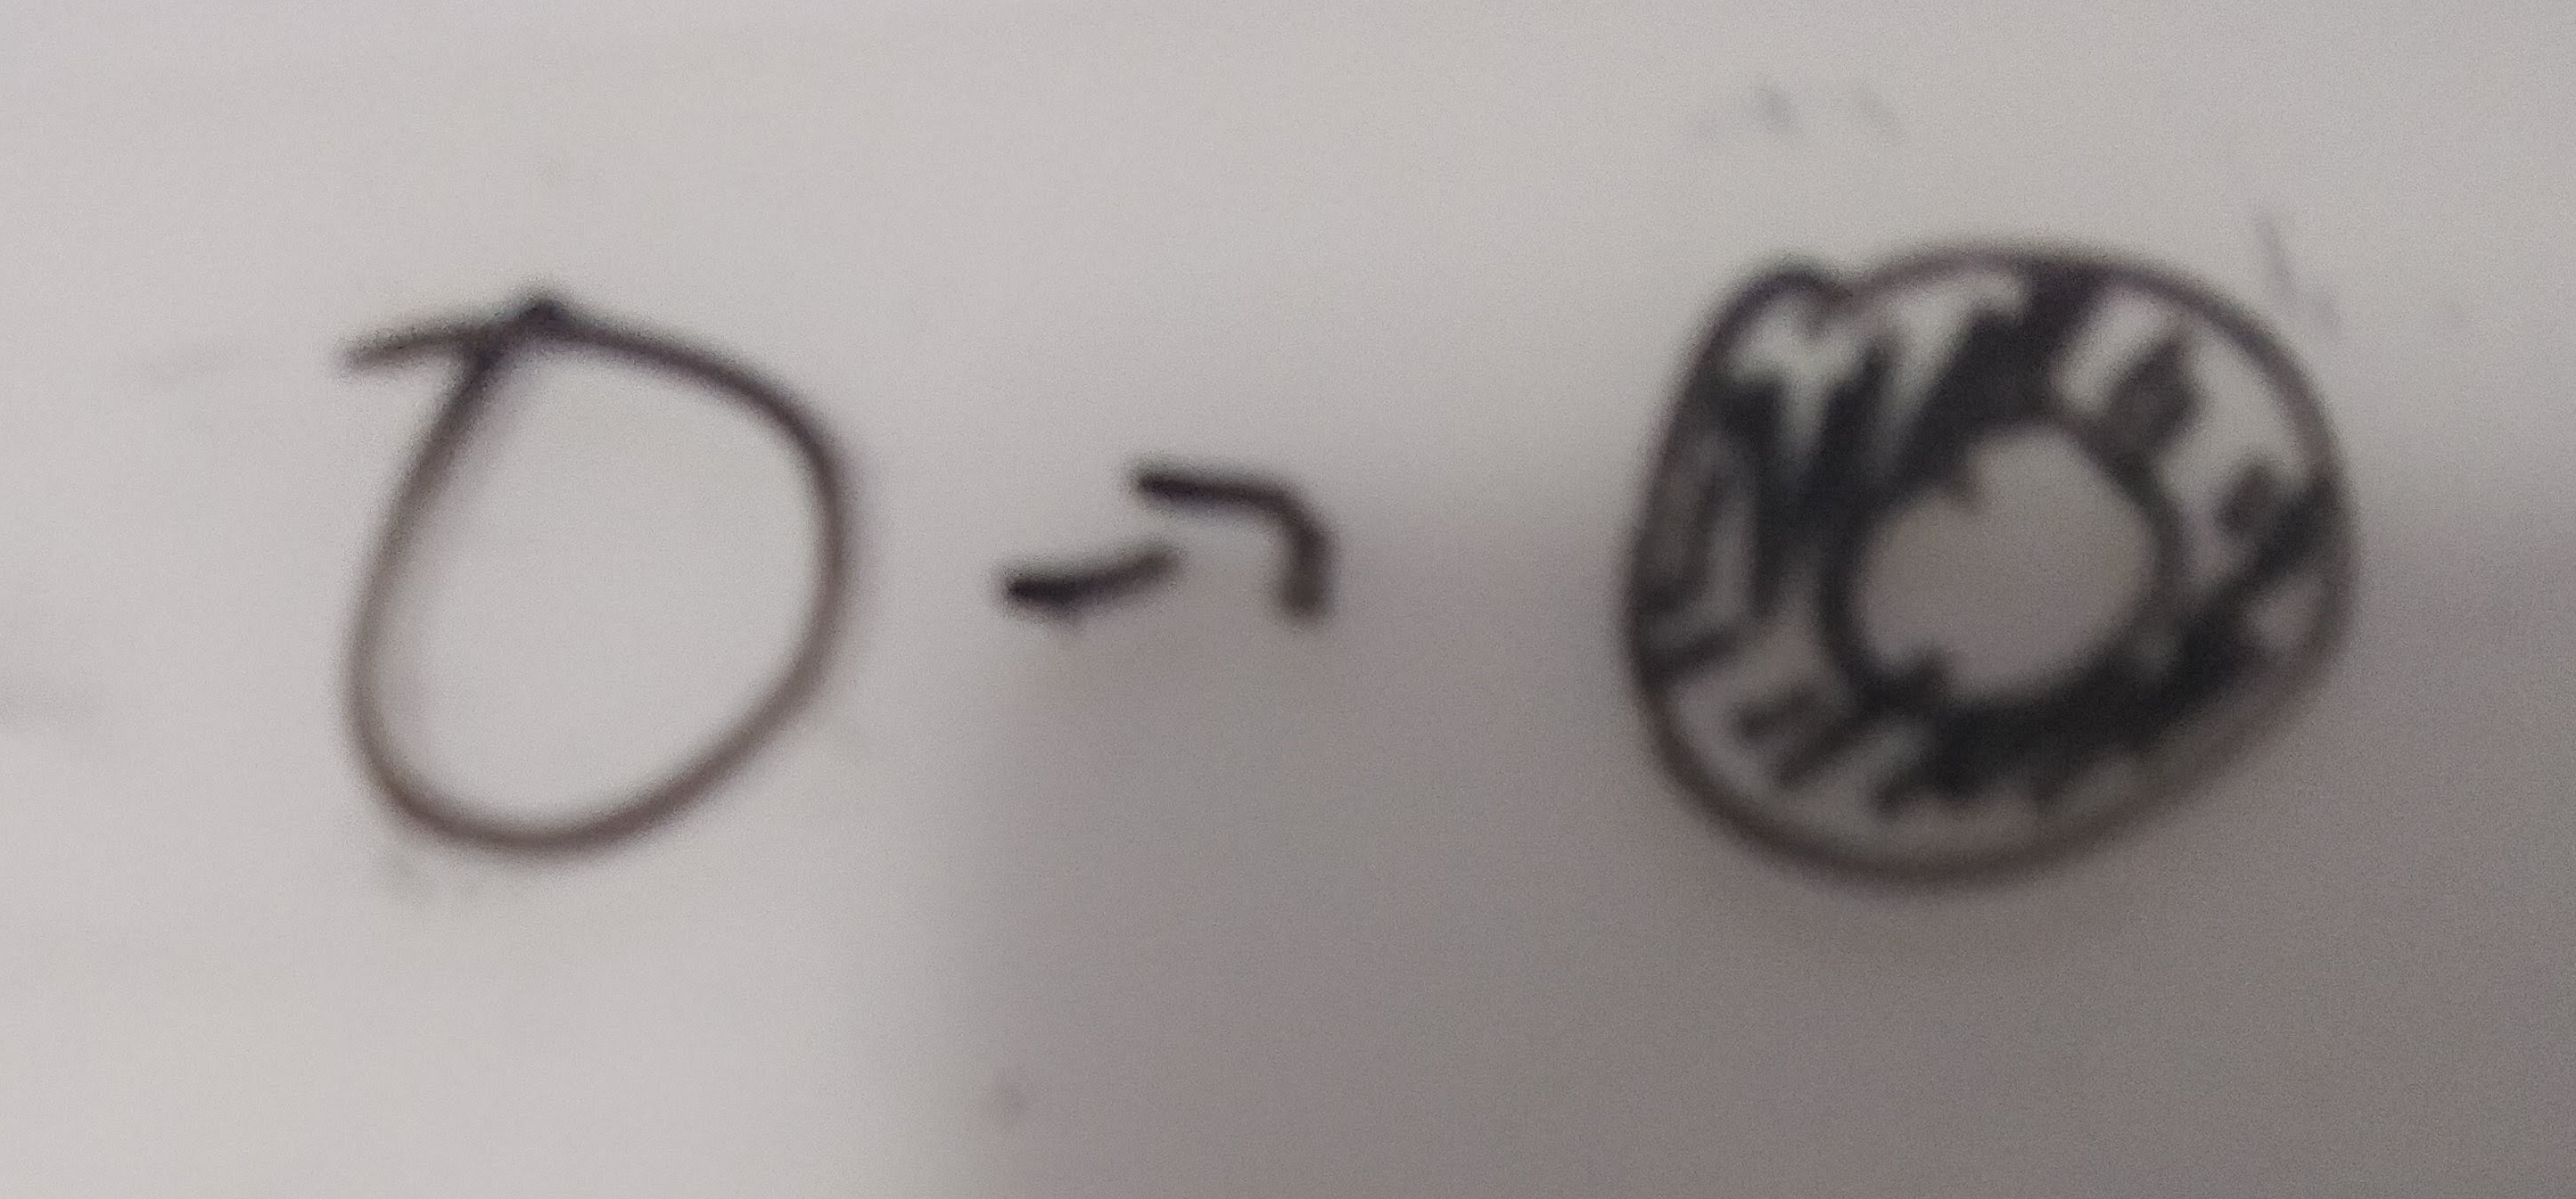
\includegraphics[width=\textwidth]{figures/math/diff_type_q.png}
    \label{fig:artist_mark_change}
\end{figure}

Many $\mu_{i}$ are graphical parameters that do not apply to the whole glyph, such as edge thickness in figure~\ref{fig:artist_mark_change}. 

%%% rework this sentence
In these situations, not all  $\rho$ in $\Gamma(H)$ will support these parameters; instead we define an action on the output graphic $Q(\Gamma(V)) \in \Gamma(H)$ since by definition every section $\mu$ will have a corresponding $\rho$.

We then define the constraint on $Q$ such that if $Q$ applied to two sections $\mu, \mu\prime$ generate the same graphic $\rho$, then the output of both sections acted on by the same monoid $m$ must also be the same.    

Lets call the visual encodings $\Gamma(V)=X$ and the graphic $Q(\Gamma(V))=Y$. If $\forall m \in M$ and $\forall \mu, \mu^\prime \in X$, 
\begin{equation}
Q(\mu) = Q(\mu^\prime)\implies Q(m\circ\mu) = Q(m\circ\mu^\prime)
\end{equation}
then a group action on $Y$ can be defined as $m\circ \rho = \rho^\prime$ where $\rho^\prime=Q(g\circ \mu)$ with $\mu \in Q^{-1}(\rho)$. 

Given  
\begin{itemize}
    \item $P = \{xpos, ypos, color, thickness\}$
    \item $\mu = {0,0,0, 1}$
    \item  $Q(\mu)=\rho$ generates a piece of the thin circle in figure~\ref{fig:artist_mark_change}
\end{itemize}

the constraint on $Q$ means that the translation $m=\{e, e, e, x+2\}$ applied to $\mu$ such that $\mu^\prime=\{0,0,0,3\}$ has an equivalent action on $\rho$ that causes $Q(\mu\prime)$ to be equivalent to the thicker circle in figure~\ref{fig:artist_mark_change}.


\paragraph{Example: Invalid Q}
\textcolor{blue}{Insert some degenerate Q that generates an inconsistent glyph}


Check a well defined map $M\times Y \rightarrow Y$.


constraint: inputs go to same o
utput means changes to inputs mean same changes to output

\paragraph{Graphical Marks}
To output a mark  \cite{bertinIIPropertiesGraphic2011,carpendaleVisualRepresentationSemiology}, $Q$ is called with all the regions $s$ that map back to a set of connected components $J \subset K$:
\begin{equation}
J = \{j \in K \text{ s. t. } \exists \gamma \text{ s.t. } \gamma(0)=k \text{ and }\gamma(1)=j\}
\end{equation}
where the path\cite{ConnectedSpace2020}  $\gamma$ from $k$ to $j$ is a continous function from the interval [0,1].

We define the mark as the graphic generated by $Q(S_j)$

\begin{equation}
    \begin{tikzcd}
        H \arrow[r, shift left] & S_j \arrow[rr, "\xi(s)", shift left] \arrow[l, "\rho(S_j)"] &  & J_{k} \arrow[ll, "\xi^{-1}(J)"]
        \end{tikzcd}
    \label{eq:mark}
\end{equation}

in terms of $K$ because mark is a semantic term denoting the graphic representation of the data.

\subsubsection{Sample Qs}
%rewrite as alpha/beta 
In this section we formulate the minimal Q that will generate distinguishable graphical marks: non-overlapping scatter points, a non-infinitely thin line, and a simple heatmap. 

\paragraph{Q: scatter plot}\mbox{} \\
\label{sec:artist_example_scatter}
\begin{figure}[ht!]
    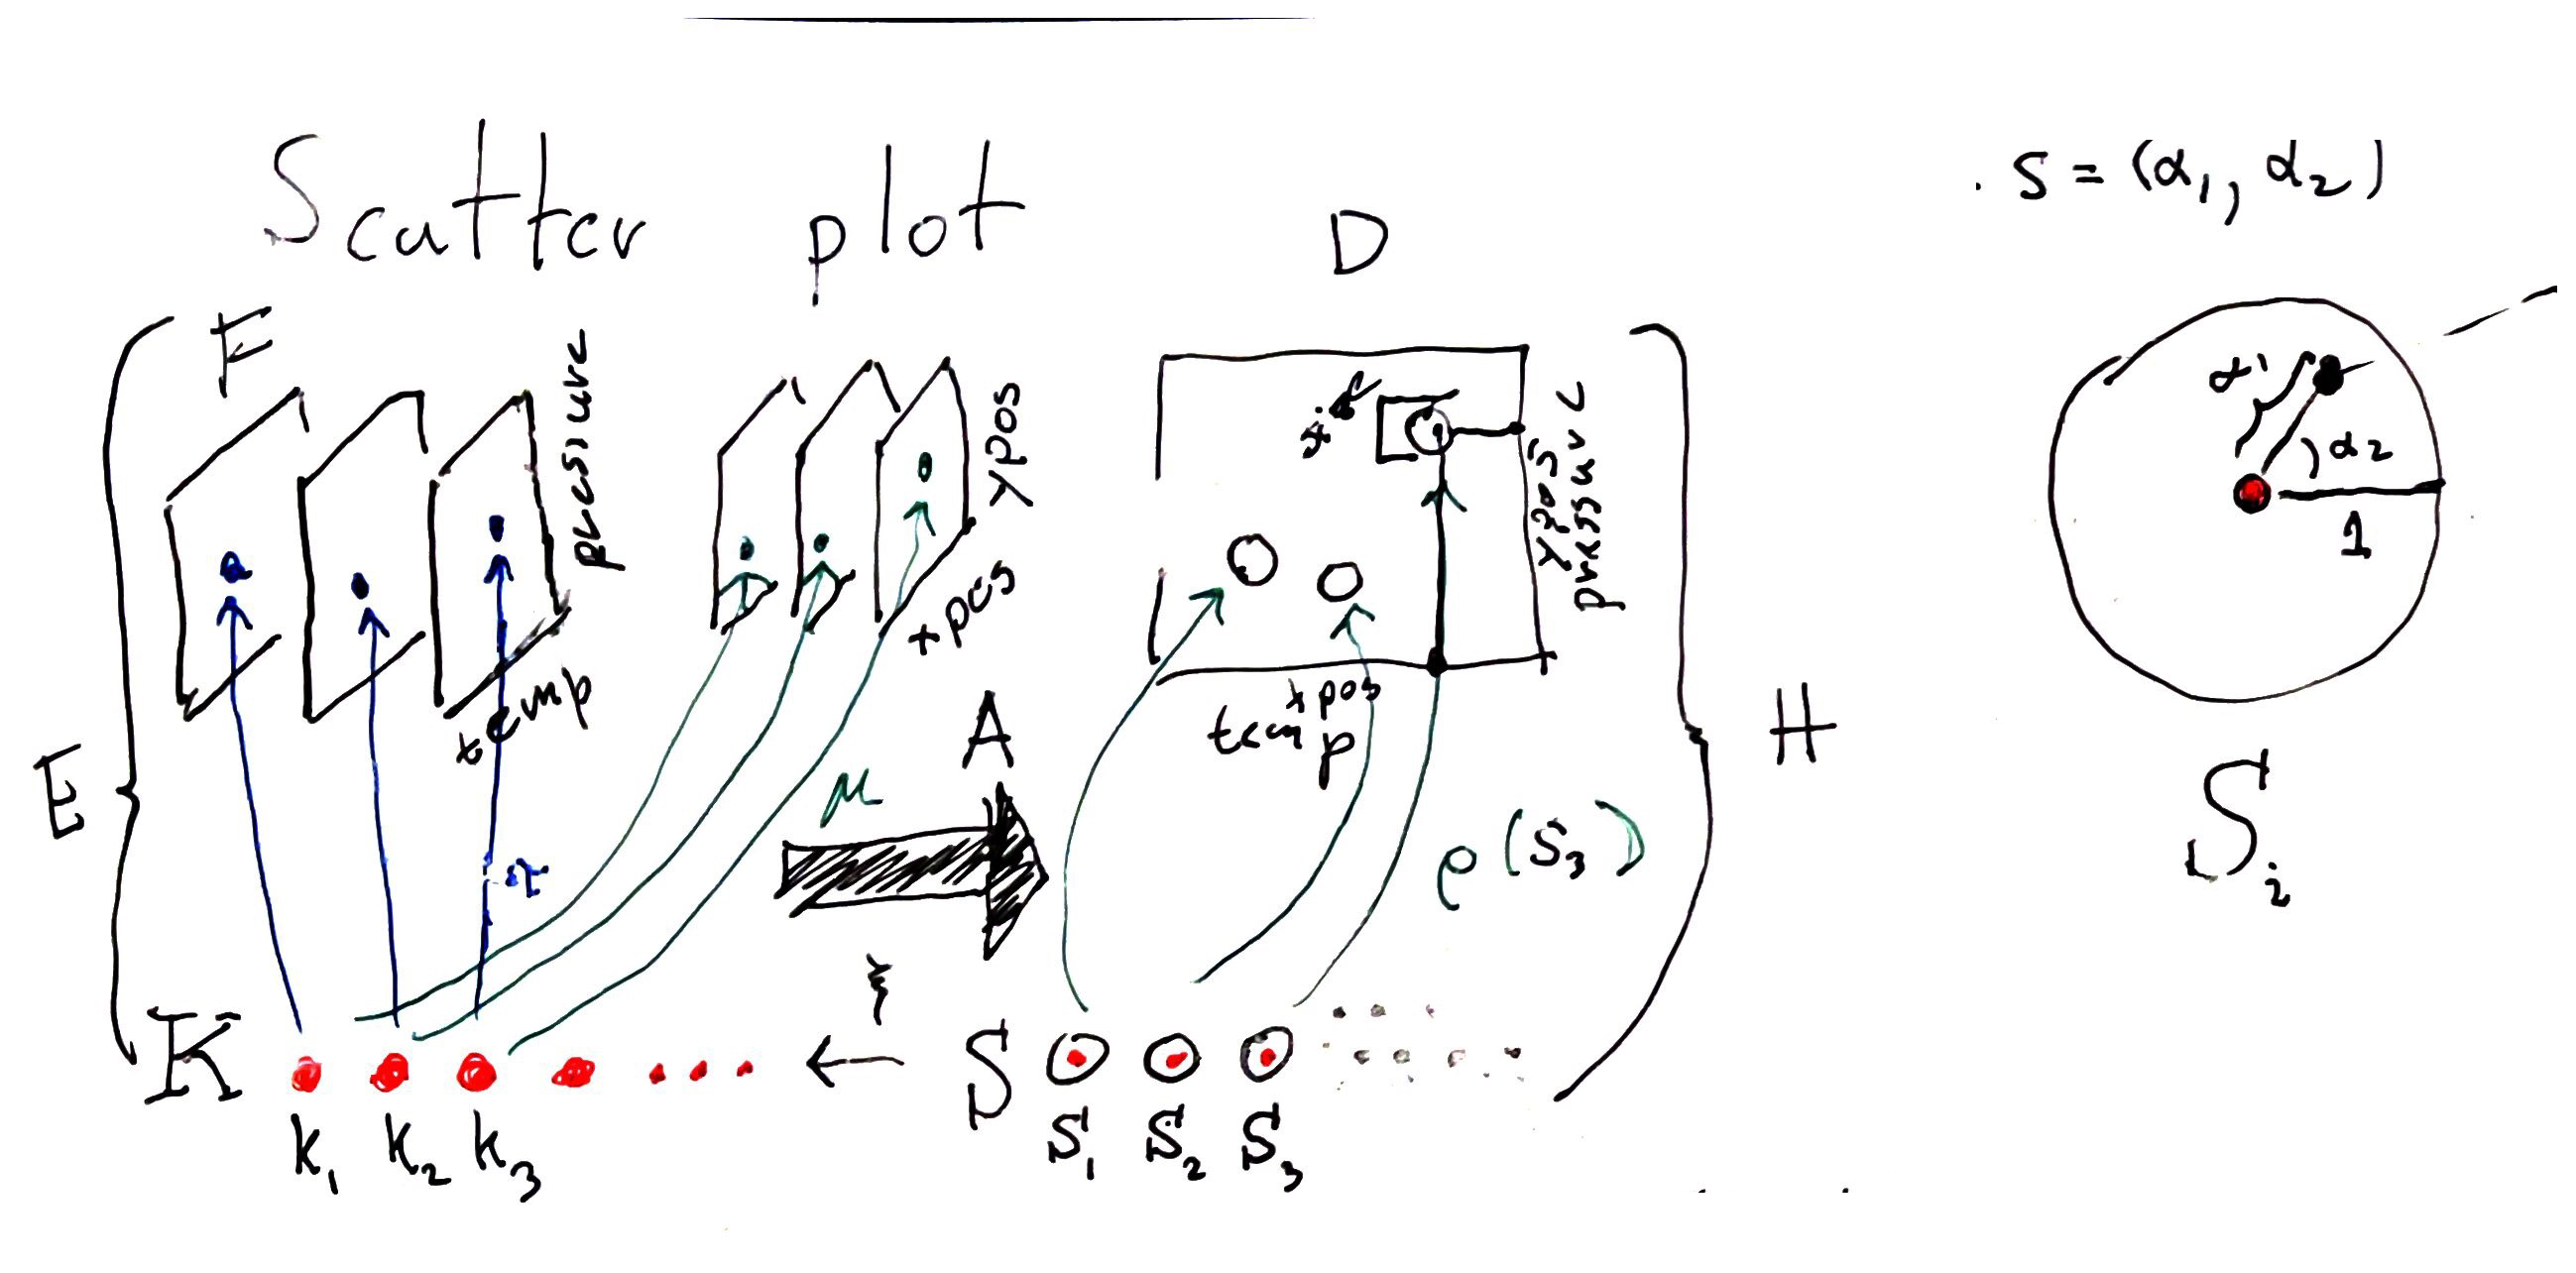
\includegraphics[width=\textwidth]{figures/math/scatter.png}
    \label{fig:artist_scatter}
\end{figure}

\begin{equation}
Q(xpos, ypos)(\alpha_{1}, \alpha_{2}) 
\end{equation}

Given a defaut color of black, $\rho_{RGB} = (0,0,0)$. The position of this swatch of color can be computed relative to the location on the disc $S_{i}$ as shown in figure~\ref{fig:artist_scatter}:
\begin{align}
x &= size\bullet \alpha_1 \bullet \cos(\alpha_2) + xpos\\
y &= size\bullet \alpha_1 \bullet \sin(\alpha_2) + ypos
\end{align}

such that $\rho(s) = (x, y, 0, 0, 0)$ where $s$ is the region in $H$. 

\paragraph{Q: line plot}\mbox{} \\
\label{sec:artist_example_line}
\begin{figure}[ht!]
    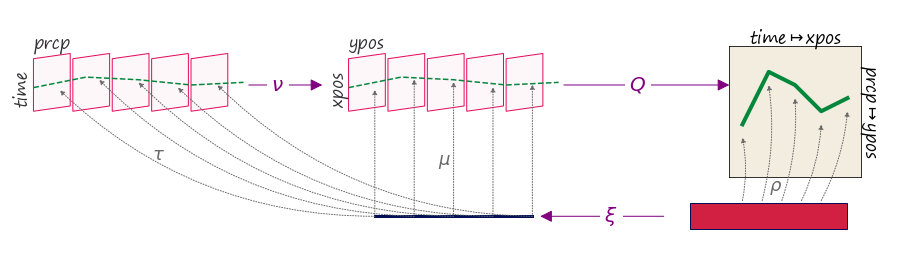
\includegraphics[width=\textwidth]{figures/math/line.png}
    \label{fig:artist_line}
\end{figure}

The line plot shown in fig~\ref{fig:artist_scatter} exemplifies the need for the jet discussed in section~\ref{sec:sheaf_stalk}
(needs the normal to push up/down against the normal)

\begin{equation}
    Q(xpos, \hat{n_{1}}, ypos, \hat{n_{2}})(\alpha_1, \alpha_2)
\end{equation}

where the magnitude of the thickness is 
\begin{equation}
    \lvert n \rvert = \sqrt{{n_{1}}^2 + {n_{2}}^2}
\end{equation}
such that the components are 
\begin{equation}
    \hat{n_{1}} = \frac{n_1}{\lvert n \rvert}, \; \hat{n_{2}} = \frac{n_2}{\lvert n \rvert}
\end{equation}
    
%% only alpha1 exists on the data side
which yields components of $\rho(s)$:
\begin{align}
 x = xpos(\xi(\alpha_1)) &+ \alpha_2\hat(n_1)(\xi(\alpha_1)) \\
 y = ypos(\xi(\alpha_1)) &+ \alpha_2\hat(n_2)(\xi(\alpha_2)) 
\end{align}


\paragraph{Q: heatmap}\mbox{} \\
\label{sec:artist_example_heatmap}
\begin{figure}[ht!]
    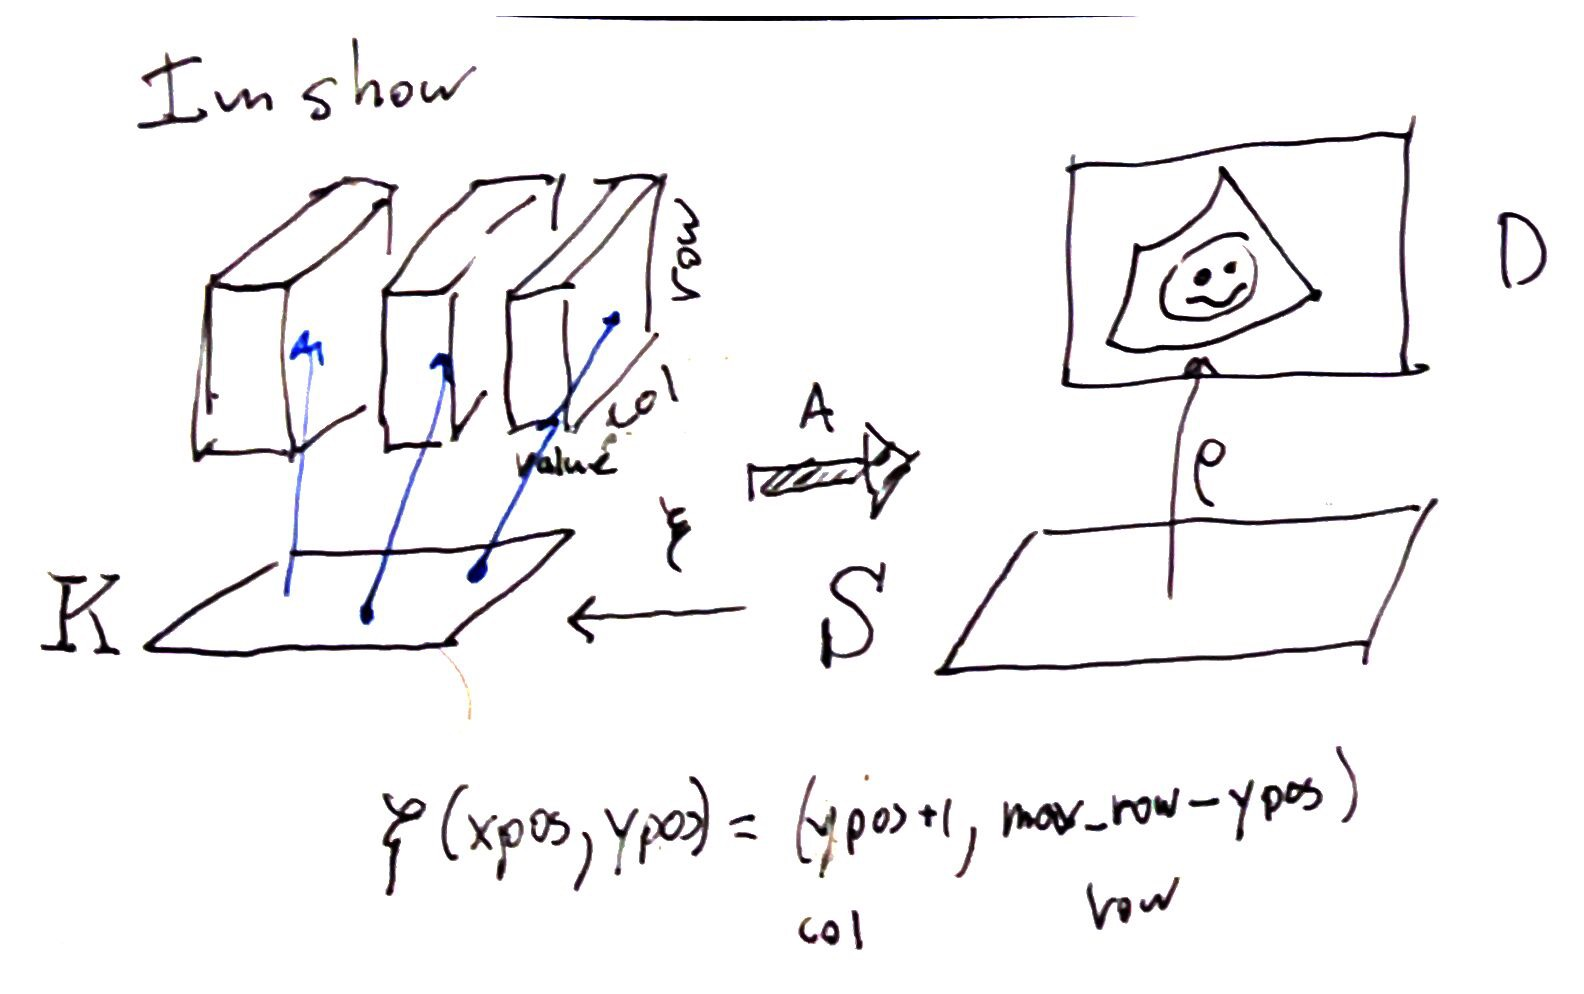
\includegraphics[width=\textwidth]{figures/math/heatmap.png}
    \label{fig:artist_heatmap}
\end{figure}
The heatmap in figure~\ref{fig:artist_heatmap} 
\begin{equation}
Q(xpos, ypos, color)
\end{equation}
has in the simple case a direct lookup into $K$ to obtain the $\mu = (x,y,c)$ values that are mapped into 
(arrays are upside down, x is y, is x) - $\xi$ is about translating indices from data to visual alignment
\begin{align}
D_{RGB} &= color(\xi(\alpha_1, \alpha_2))
D_x & = xpos(\xi(\alpha_1, \alpha_2))
D_y &= ypos(\xi(\alpha_1, \alpha_2))
\end{align}
through $\rho$. 


\subsection{Making the fiber bundle computable}
\label{sec:triangulization}

\begin{figure}[ht!]
    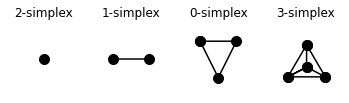
\includegraphics{figures/math/simplex.png}
    \caption{Simplices can encode the connectivity of the data, from fully disconnected (0 simplex) records to all records are connected to at least 3 others}
    \label{fig:triangle_simplex}
\end{figure}

One way to build flexible $\xi$ is to choose a consistent way of representing $K$. In our draft implementation of the data as fiber bundle model, we triangularize $K$ using complexes of the simplicies shown in figure~\ref{fig:triangle_simplex} such that $\xi$ consistently yields some combination of vertexes, edges, and faces. This gives a common data indexing structure on which to build components that could potentially be reused across $Q$.

By using simplicies, we can then encode the following indexing structure on $\tau$
\begin{align*}
    \textbf{vertexes}\;& \tau(k) \text{k= vertex id}\\
    \textbf{edges}\;& \tau(k,\alpha), \text{k = edge id, $\alpha$ = distance along edge} \\
    \textbf{faces}\;& \tau(k,\alpha, \beta), \text{k = face id, $\alpha$ = x on face, $\beta$ = y on face}
\end{align*}

which $\xi$ can use as part of its mapping from visual space back to data space. Path connected components are then sections where $\tau(k_{i},1) = \tau(k_{j},0)$ or the edges of the faces align.  

\subparagraph{Example: Mobius Strip}\mbox{}\\
\begin{figure}[ht!]
    \label{fig:data_base_transition}
    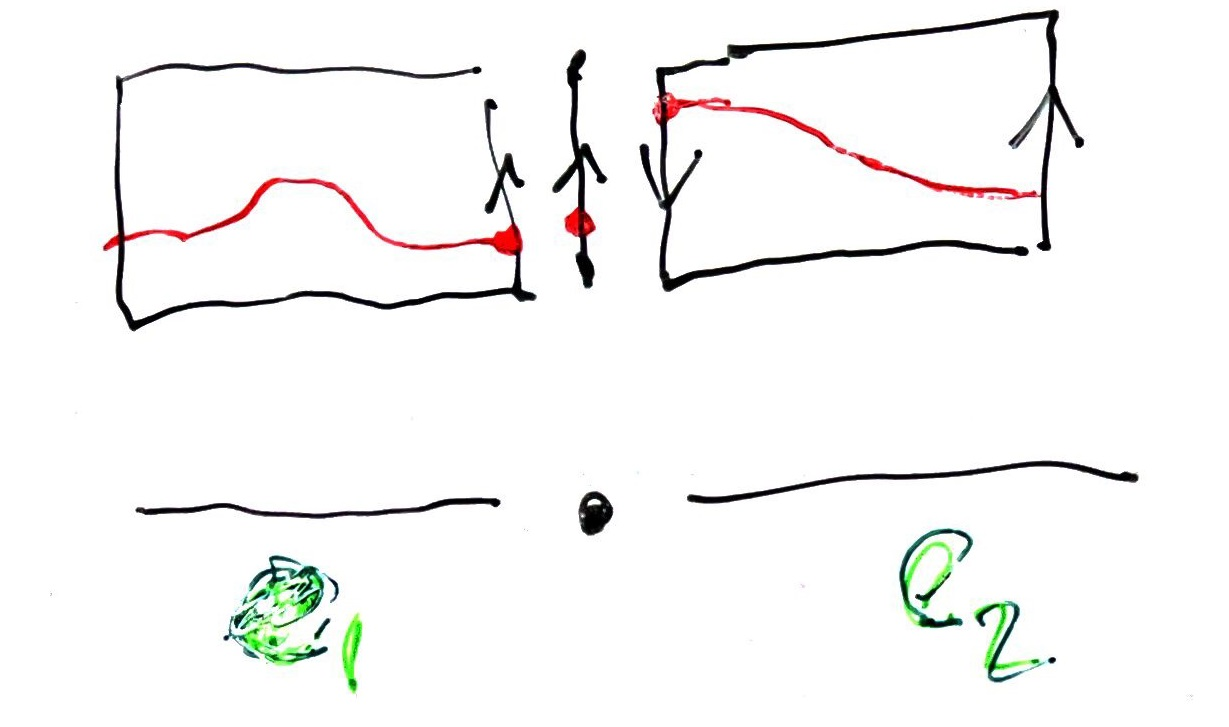
\includegraphics[width=\textwidth]{figures/math/transition_functions.png}
    \caption{Many non-trivial spaces can be made locally trivial by dividing $E$ into locally trivial subspaces and defining transition functions between the edges on K for how to glue the two subspaces such that the sigmas are continuous.}
\end{figure}

 An example of a non-trivial fiber bundle is a mobius strip\cite{find the citation for why};

In figure ~\ref{fig:data_base_transition}, the mobius strip is cut into two rectangular base spaces over $K=\{e_1, e_2\}$. We define transition functions from the fiber to the fiber along the edges of the rectangles such that we can glue these rectangles together to reform the mobius strip. A constraint we impose on the transition functions is that the monoid actions are commutative
%monoid action m*f\mapsto delta(mf)= m*delta(f)

\subparagraph{Example: Torus}\mbox{}\\
\begin{figure}[ht!]
    \label{fig:triangle_torus}
    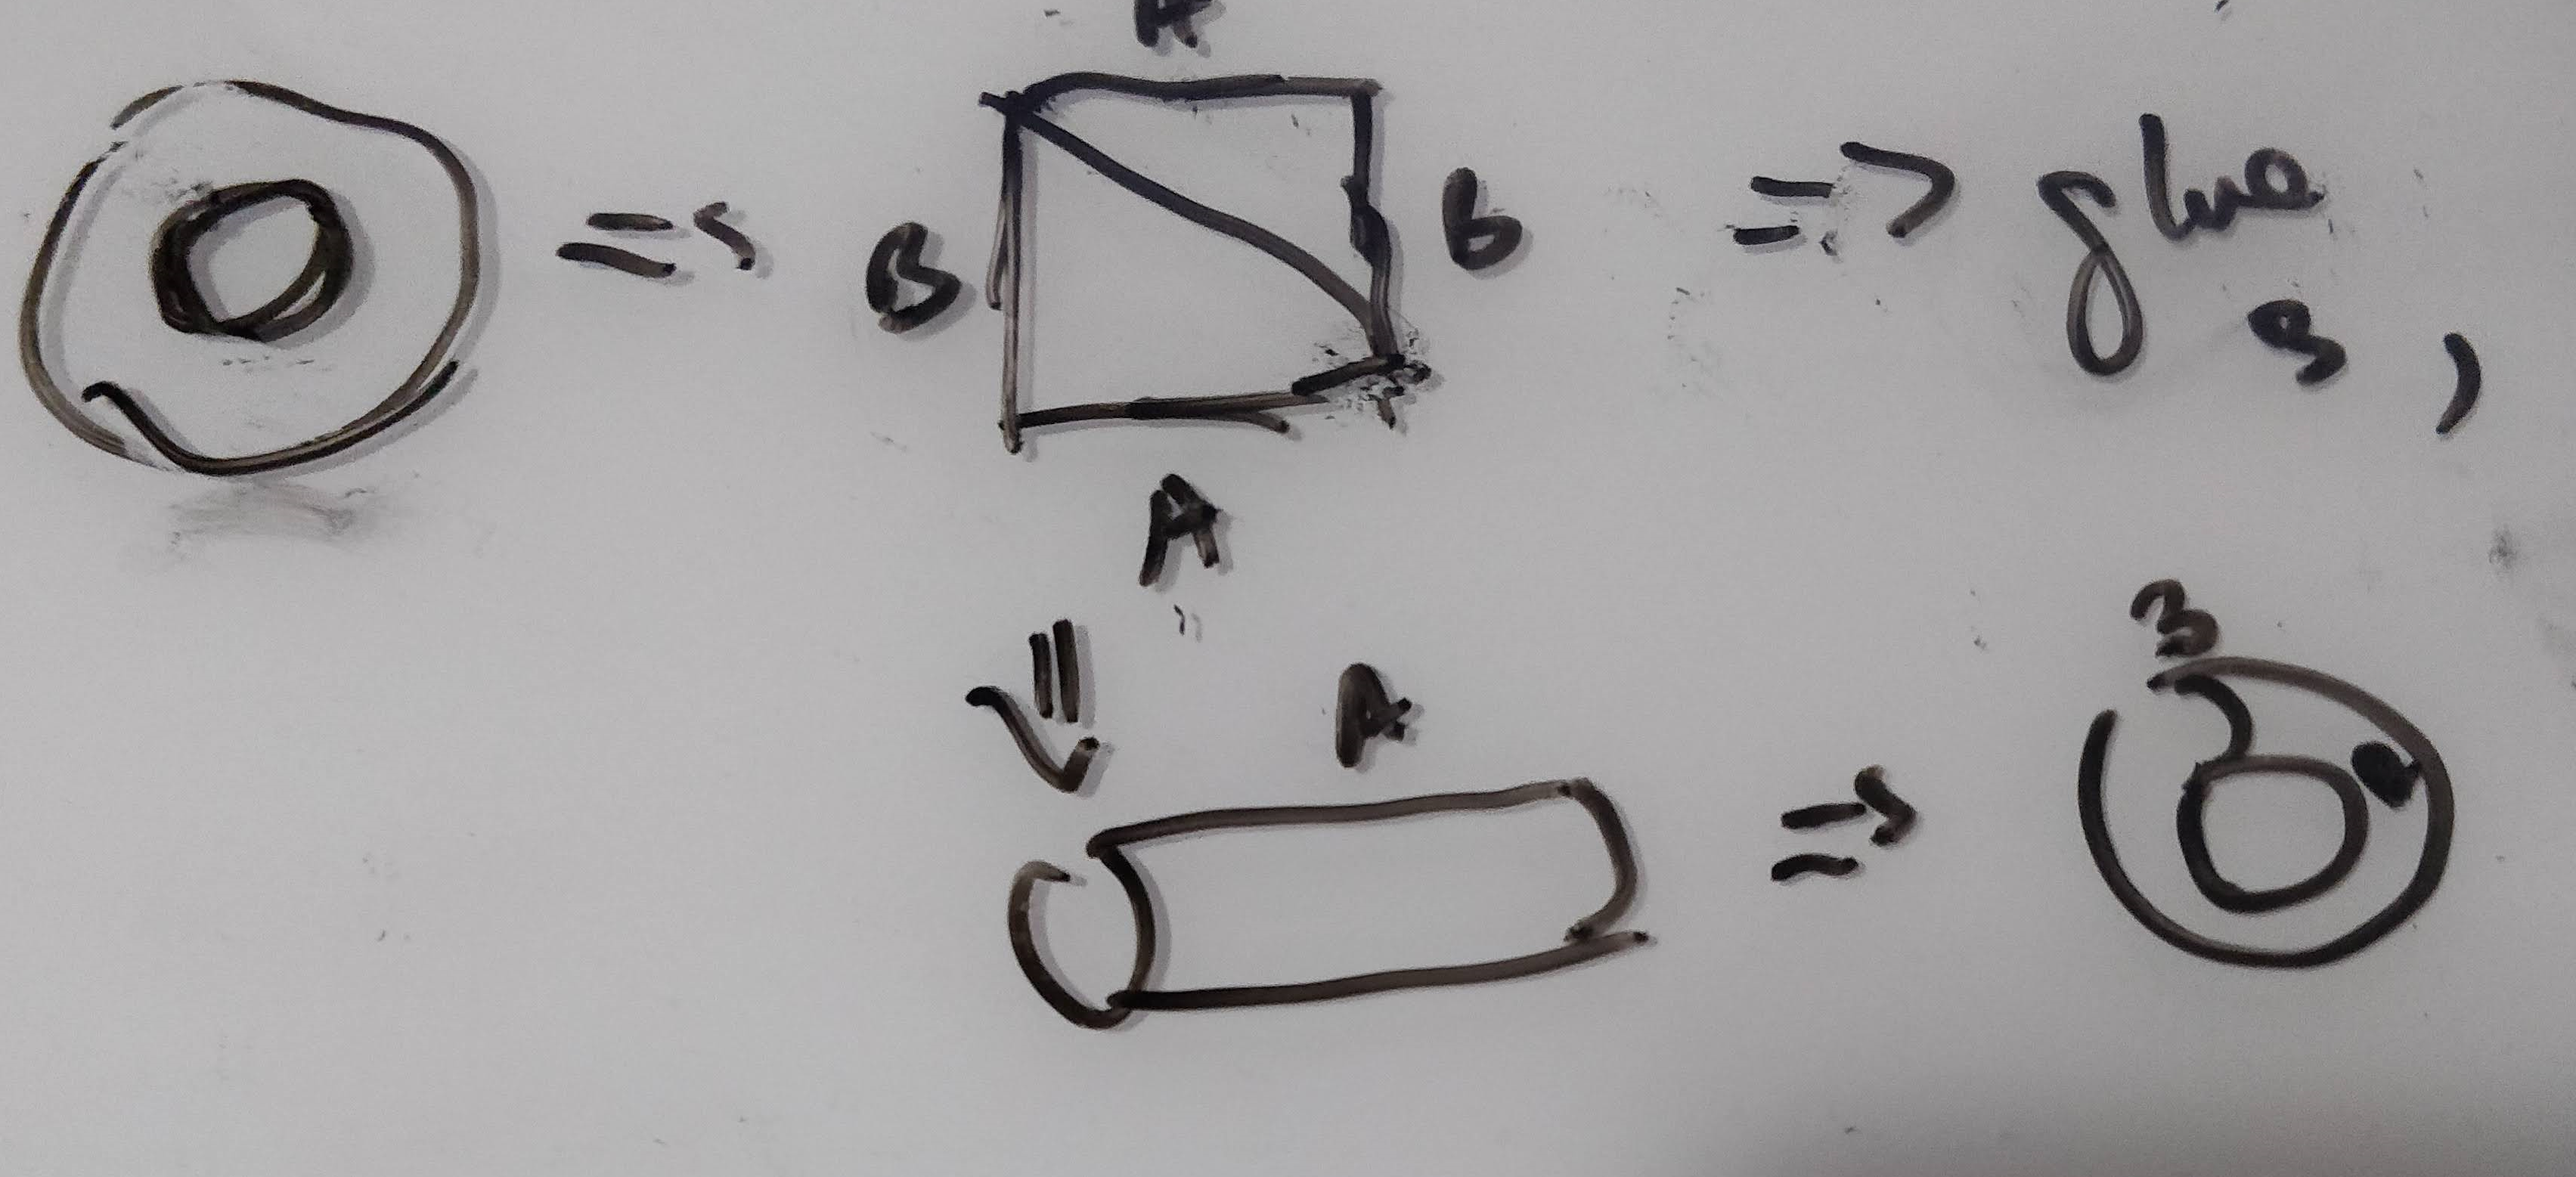
\includegraphics[width=\textwidth]{figures/math/triangle_torus.png}
    \caption{Representation of the base space $K$ of a toridal total space $E$ as two connected 2-simplices.}
\end{figure}

Given data that lies on the toroidal space shown in figure~\ref{fig:triangle_torus}, the torus $E$ base space $K$ can be implemented as a simplacial complex of two 2-simplexes. We unfold the torus into the two triangles that compose the square; the sections on these triangles are $\tau(triangle id k, \alpha, \beta)$. We also put transition functions on the edges such that $A$ can be glued to $A^\prime$ and $B$ to $B^\prime$ to reconstruct the torus. 

\subsubsection{Visual Idioms: Equivalance class of artists}
As formulated above, every artist function $A$ has fixed $\nu$ and generates a distinct graphic $\rho$. It is unfeasible to implement $A$ for every single graphic; instead we implement the equivalence class of artists $\{A \in A^\prime: A_{1} \equiv A_{2}\}$ which is $Q:\Gamma(V) \rightarrow \Gamma(H)$. 

%% Well maybe. I think this is where required components comes in. There is some minimal V where if you didn't have those variables you wouldn't call it a scatter plot .... something like xpos,ypos with K just a descrete set.
%% so V probably can be any V that contains that sub-bundle
%% so if bubble plot is not the same as scatter plot, and something where the colors change based on data is not scatter plot then it is the equivalent class of something with that minimal bundle.
%% But then if you want to include ANYTHING that also maps with X-Y ... then you hit "direct limits" where you limit over all possivle V_big containing V_minimal
%% You still get a map on some A_minimal -> A_big
%% If you know how to visualize with more variables .. you can always fix them.
\end{document}